\documentclass[]{article}

% Imported Packages
%------------------------------------------------------------------------------
\usepackage{amssymb}
\usepackage{amstext}
\usepackage{amsthm}
\usepackage{amsmath}
\usepackage{enumerate}
\usepackage{fancyhdr}
\usepackage[margin=1in]{geometry}
\usepackage{graphicx}
\usepackage{float}
\usepackage{placeins}
%\usepackage{extarrows}
%\usepackage{setspace}
%------------------------------------------------------------------------------

% Header and Footer
%------------------------------------------------------------------------------
\pagestyle{plain}  
\renewcommand\headrulewidth{0.4pt}                                      
\renewcommand\footrulewidth{0.4pt}                                    
%------------------------------------------------------------------------------

% Title Details
%------------------------------------------------------------------------------
\title{Deliverable \#2}
\author{SE 3A04: Software Design III -- Large System Design}
\date{}                               
%------------------------------------------------------------------------------

% Document
%------------------------------------------------------------------------------
\begin{document}

\maketitle
\noindent{\bf Tutorial Number:} T01\\
{\bf Group Number:} G02 \\
{\bf Group Members:}
\begin{itemize}
  \item Omer Karo
  \item Ahsan Muzammil
  \item Jake Finlay
  \item Ethan Walsh
  \item Rebecca Di Filippo
  \item Abdallah Alqashqish
\end{itemize}

\section*{IMPORTANT NOTES}
\begin{itemize}
  %	\item You do \underline{NOT} need to provide a text explanation of each diagram; the diagram should speak for itself
  \item Please document any non-standard notations that you may have used
        \begin{itemize}
          \item \emph{Rule of Thumb}: if you feel there is any doubt surrounding the meaning of your notations, document them
        \end{itemize}
  \item Some diagrams may be difficult to fit into one page
        \begin{itemize}
          \item Ensure that the text is readable when printed, or when viewed at 100\% on a regular laptop-sized screen.
          \item If you need to break a diagram onto multiple pages, please adopt a system of doing so and thoroughly explain how it can be reconnected from one page to the next; if you are unsure about this, please ask about it
        \end{itemize}
  \item Please submit the latest version of Deliverable 1 with Deliverable 2
        \begin{itemize}
          \item Indicate any changes you made.
        \end{itemize}
  \item If you do \underline{NOT} have a Division of Labour sheet, your deliverable will \underline{NOT} be marked
\end{itemize}

\newpage
\section{Introduction}
\label{sec:introduction}
% Begin Section

\subsection{Purpose}
\label{sub:purpose}
% Begin SubSection
\indent\indent This document provides a high level overview of the DealCheck system architecture, including high level design considerations of the system, as well as design considerations for various subsystems. This document is intended for internal DealCheck stakeholders, including project managers, software developers, domain experts, and DealCheck team members/investors. It is recommended that DealCheck deliverable 1 is read prior to this, and the reader has some basic software technical knowledge.
% End SubSection

\subsection{System Description}
\label{sub:system_description}
% Begin SubSection
\indent\indent The overall DealCheck system follows a Blackboard (BB) style architecture, with various subsystems adopting either a BB or repository style design architecture.
The BB architecture supports multiple agents or "experts" that contribute toward the evaluation of car deals, with each agent operating independently to add insights to the shared Blackboard, which acts as the central data store.
Additionally, the repository style design architecture is used for subsystems that require concurrent access to data, particularly in areas like account management. This architecture is specialized for handling high-complexity data processing, ensuring that user account information and car valuation reports are securely and efficiently managed in DealCheck.
% End SubSection

\subsection{Overview}
\label{sub:overview}
% Begin SubSection
\indent\indent Section 2 presents an Analysis Class Diagram. In Section 3, the document goes into the architectural design of the system, as well as discusses considered alternatives, and reasoning behind design decisions. Next, in Section 4, Class Responsibility Collaboration (CRC) Cards are presented to understand the inside of the classes, their responsibilities, and the interactions between classes. Lastly Section A, is the division of labour section where we discuss who focused on which parts.

% End SubSection

% End Section

\pagebreak

\section{Analysis Class Diagram}
\label{sec:analysis_class_diagram}
% Begin Section
\begin{figure}[H]
  \centering
  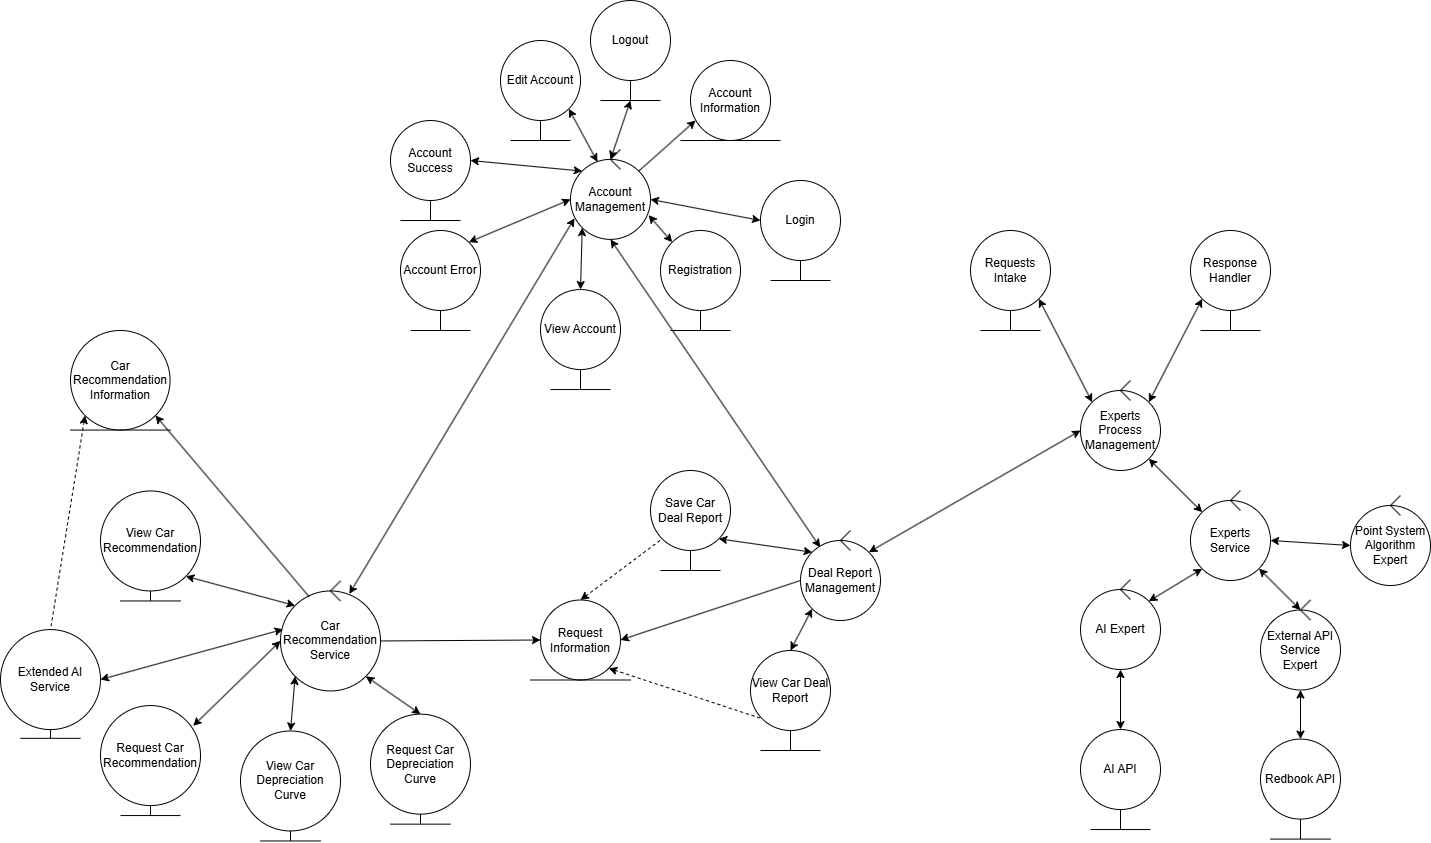
\includegraphics[scale=0.35]{3A04_acd.png}
  \caption{Analysis Class Diagram}\label{Fig:2.1}
\end{figure}
% End Section

\pagebreak

\section{Architectural Design}
\label{sec:architectural_design}
% Begin Section

\subsection{System Architecture}

\begin{figure}[H]
  \centering
  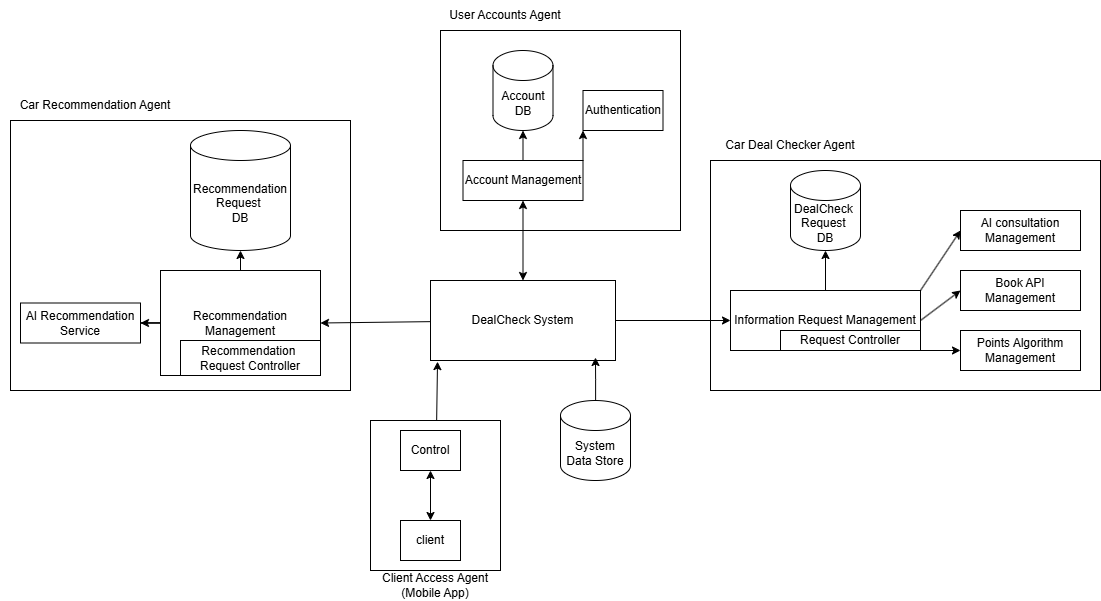
\includegraphics[scale=0.45]{3A04_sys2.png}
  \caption{System Diagram}\label{Fig:2.1}
\end{figure}

\label{sub:system_architecture}
% Begin SubSection

\indent \indent The DealCheck System will adopt a Data-Centered architecture, specifically the Blackboard architecture style. The system’s core 
functionality is managed through the Request Controller, which is accessed via the Client Access. The Client Access is responsible for controlling 
the application's user interface. The DealCheck Request Database will act as the central ‘data store’ used in Blackboard architecture, while each 
of the subsystems described below will interact with the main DealCheck System to accomplish the extra functionalities of the application \\

\noindent
The core system of DealCheck comprises of three knowledge sources, also referred to as experts: \\
\begin{itemize}
    \item \textbf{AI Consultation Management}
    \item \textbf{Book API Management}
    \item \textbf{Points Algorithm Management}
\end{itemize}
\noindent
These components collectively perform the primary function of the application—determining whether a car deal is favorable. \\

\noindent The following table summarizes the purpose and architectural style of each subsystem:
\FloatBarrier
\begin{table}[H]
  \centering
  \begin{tabular}{|p{5cm}|p{7cm}|p{3cm}|}
    \hline
    \textbf{Subsystem}        & \textbf{Purpose}                                                                       & \textbf{Architectural Style} \\
    \hline
    Account Management        & Users manage, modify, and create account-related data.                                 & Repository                   \\
    \hline
    DealCheck System    & Users query the system for information on a car deal as well as view and save results. & Blackboard                   \\
    \hline
    Recommendation Management & Users obtain recommendations on car purchases.                                         & Blackboard                   \\
    \hline
  \end{tabular}
  \label{tab:dealcheck_subsystems}
\end{table}
\FloatBarrier
\noindent
Further subsystem descriptions are provided in Section 3.2 of this document. \\
\newline
This system will also employ four databases:
\begin{itemize}
  \item The \textbf{Account Database} will hold user information such as usernames and passwords.
  \item The \textbf{Recommendation Request Database} will store records from user queries for car recommendations.
  \item The \textbf{DealCheck Request Database} will act as the central data store for the entire application.
\end{itemize}

DealCheck’s architecture utilizes both the Repository and Blackboard systems. For the overall system, the Blackboard architecture is used since it will allow for separation of application components (see the above subsystems) that may each independently work within the application. The DealCheck Request Database will also store application wide data, including user interface information and user request information. This central data store will invoke the correct subsystems based on the request. \\

The DealCheck System is a blackboard architecture because there is not one universally correct answer for the valuation of a vehicle. Therefore, multiple knowledge sources must be consulted and integrated together to provide a quality response. This aligns with the Blackboard style, where the data store is active and calls upon the relevant knowledge sources to answer a query. This was chosen over other architectural systems such as Batch Sequential and Repository due to the problem’s structure. Rating of a vehicle deal is non-deterministic and yields the best results when multiple agents are consulted, therefore Blackboard is the optimal choice.\\

The second architecture style used in this application is Repository. This style is frequently used in database management systems, where frequent modification to data is required. This is similar to the needs of the Account Management System. Additionally, the data store is passive rather than active, which is suitable for the account management system which will only be modified by the clients accessing. The repository style was chosen over other data-centered architectures such as blackboard, which is more suited for solving non-deterministic problems. This is not the case, therefore the repository is used. Data Flow architectures were also not selected since this system’s activities are not a series of transformations on data sets. Returning to the benefits of the repository, a key strength is its well-suitedness for applications needing data integrity. This is a top priority of an account management system, since sensitive data such as usernames and passwords must be secure and maintain a high level of integrity.\\

We considered using Batch Sequential from the data flow architecture to handle car deal requests, where a user submits a request and DealCheck processes it through the main system. However, this approach was not suitable since the system requires real-time responses, whereas batch processing introduces delays. Users expect instant feedback on deal evaluations, and waiting for a batch cycle would be impractical. Additionally, Batch Sequential has low throughput due to its rigid, sequential processing steps, making it inefficient for an application with multiple users.\\

Another alternative we explored was Pipes and Filters for the DealCheck main system. However, this architecture lacks the flexibility needed for non-deterministic car deal evaluations. Since different deals may require varying types of analysis depending on the input and expert consulted, a fixed sequence of steps would not be ideal. Pipes and Filters work best for structured data transformations, whereas DealCheck's subsystems require dynamic data integration from multiple sources, which this architecture is not well-suited for.\\

We also considered the Process-Control architecture but ultimately eliminated it because it is designed for continuous monitoring and real-time feedback loops, such as temperature regulation systems. Since DealCheck operates on user-initiated queries, rather than ongoing system monitoring, Process-Control was unnecessary for this application.\\
% End SubSection

\subsection{Subsystems}
\label{sub:subsystems}
% Begin SubSection

Dealcheck’s primary system has been subdivided into three subsystems: Account Management, Main DealCheck System, and Car Recommendation. \\

Account Management will serve as the center for all related information and queries to account details. This will include storing information such as usernames and passwords. Functions of this system will primarily be for modification of this information, for example, a function to reset a user’s password. \\

The DealCheck main System will serve as the core functionality of the DealCheck app, enabling users to view previous car deal reports, save new reports, and request car deal evaluations. It interacts with the Account Management subsystem to retrieve a user's past queries by linking their account information with the app's query history. Additionally, it interacts with the Account Management subsystem to save car deal reports to the corresponding user accounts. This main system also handles car deal evaluation requests, collaborating with controllers like Request Controller to process requests, select the appropriate experts based on user input, and generate detailed car deal reports. Finally, this main system saves the results of the user's car deal evaluation request in the DealCheck Reqeust Database. \\

The Car Recommendation Service subsystem is our innovative feature, responsible for handling user requests related to car recommendations and depreciation curves, displaying results, and generating these insights. It collaborates with the Account Management subsystem to authenticate users and grant access to its functionalities. When a user requests car recommendations based on their specific scenario, the subsystem uses an AI API Service to generate personalized suggestions. Additionally, it stores AI-generated car recommendations in the car recommendation information entity, which serves as a gateway to its database. The subsystem also uses the DealCheck Request Database connected with the main DealCheck System to access past car deal reports, track previously evaluated vehicles, generate depreciation curves, and link them to the corresponding car deals.

% End SubSection

% End Section

\pagebreak

\section{Class Responsibility Collaboration (CRC) Cards}
\label{sec:class_responsibility_collaboration_crc_cards}
% Begin Section
Below are all of the CRC cards for the DealCheck application.

\begin{table}[H]
  \centering
  \renewcommand{\arraystretch}{1.3} % Increases row height for better readability
  \begin{tabular}{|p{7.5cm}|p{7.5cm}|}
    \hline
    \multicolumn{2}{|l|}{\textbf{Class Name: Registration (Boundary)}}               \\
    \hline
    \textbf{Responsibility:}                         & \textbf{Collaborators:}       \\
    \hline
    Knows Account Management Controller              & Account Management Controller \\
    Handles click-event on “Make New Profile” button &                               \\
    \hline
  \end{tabular}
\end{table}
\begin{table}[H]
  \centering
  \renewcommand{\arraystretch}{1.3} % Increases row height for better readability
  \begin{tabular}{|p{7.5cm}|p{7.5cm}|}
    \hline
    \multicolumn{2}{|l|}{\textbf{Class Name: Login (Boundary)}}           \\
    \hline
    \textbf{Responsibility:}              & \textbf{Collaborators:}       \\
    \hline
    Handles click-event on “Login” button & Account Management Controller \\
    Knows Account Management Controller   &                               \\
    \hline
  \end{tabular}
\end{table}
\begin{table}[H]
  \centering
  \renewcommand{\arraystretch}{1.3} % Increases row height for better readability
  \begin{tabular}{|p{7.5cm}|p{7.5cm}|}
    \hline
    \multicolumn{2}{|l|}{\textbf{Class Name: Account Information (Entity)}}                \\
    \hline
    \textbf{Responsibility:}                               & \textbf{Collaborators:}       \\
    \hline
    Knows Account Management Controller                    & Account Management Controller \\
    Stores account information (i.e username, email, etc.) &                               \\
    \hline
  \end{tabular}
\end{table}
\begin{table}[H]
  \centering
  \renewcommand{\arraystretch}{1.3} % Increases row height for better readability
  \begin{tabular}{|p{7.5cm}|p{7.5cm}|}
    \hline
    \multicolumn{2}{|l|}{\textbf{Class Name: View Account (Boundary)}}           \\
    \hline
    \textbf{Responsibility:}                     & \textbf{Collaborators:}       \\
    \hline
    Handles click-event on “View Profile” button & Account Management Controller \\
    Displays Account Information                 &                               \\
    Knows Account Managment Controller           &                               \\
    \hline
  \end{tabular}
\end{table}
\begin{table}[H]
  \centering
  \renewcommand{\arraystretch}{1.3} % Increases row height for better readability
  \begin{tabular}{|p{7.5cm}|p{7.5cm}|}
    \hline
    \multicolumn{2}{|l|}{\textbf{Class Name: Experts Service (Controller)}}                         \\
    \hline
    \textbf{Responsibility:}                                        & \textbf{Collaborators:}       \\
    \hline
    Knows Experts Process Management Controller                     & Experts Process Management    \\
    Knows AI Expert                                                 & AI Expert                     \\
    Knows External API Service Expert                               & External API Service Expert   \\
    Knows Point System Algorithm Expert                             & Point System Algorithm Expert \\
    Handles interaction between the process manager and the experts &                               \\
    \hline
  \end{tabular}
\end{table}
\begin{table}[H]
  \centering
  \renewcommand{\arraystretch}{1.3} % Increases row height for better readability
  \begin{tabular}{|p{7.5cm}|p{7.5cm}|}
    \hline
    \multicolumn{2}{|l|}{\textbf{Class Name: AI Expert (Controller)}} \\
    \hline
    \textbf{Responsibility:} & \textbf{Collaborators:}                \\
    \hline
    Knows Experts Service    & Experts Service                        \\
    Knows AI API             & AI API                                 \\
    Processes AI queries     &                                        \\
    \hline
  \end{tabular}
\end{table}
\begin{table}[H]
  \centering
  \renewcommand{\arraystretch}{1.3} % Increases row height for better readability
  \begin{tabular}{|p{7.5cm}|p{7.5cm}|}
    \hline
    \multicolumn{2}{|l|}{\textbf{Class Name: AI API (Entity)}} \\
    \hline
    \textbf{Responsibility:} & \textbf{Collaborators:}           \\
    \hline
    Knows AI Expert          & AI Expert                         \\
    Handles AI queries       &                                   \\
    \hline
  \end{tabular}
\end{table}
\begin{table}[H]
  \centering
  \renewcommand{\arraystretch}{1.3} % Increases row height for better readability
  \begin{tabular}{|p{7.5cm}|p{7.5cm}|}
    \hline
    \multicolumn{2}{|l|}{\textbf{Class Name: External API Service Expert (Controller)}} \\
    \hline
    \textbf{Responsibility:}        & \textbf{Collaborators:}                           \\
    \hline
    Knows Experts Service           & Experts Service                                   \\
    Knows Redbook API               & Redbook API                                       \\
    Processes external API requests &                                                   \\
    \hline
  \end{tabular}
\end{table}
\begin{table}[H]
  \centering
  \renewcommand{\arraystretch}{1.3} % Increases row height for better readability
  \begin{tabular}{|p{7.5cm}|p{7.5cm}|}
    \hline
    \multicolumn{2}{|l|}{\textbf{Class Name: Redbook API (Entity)}} \\
    \hline
    \textbf{Responsibility:}            & \textbf{Collaborators:}     \\
    \hline
    Knows External API Service Expert   & External API Service Expert \\
    Handles requests to the Redbook API &                             \\
    \hline
  \end{tabular}
\end{table}

\begin{table}[H]
  \centering
  \renewcommand{\arraystretch}{1.3} % Increases row height for better readability
  \begin{tabular}{|p{7.5cm}|p{7.5cm}|}
    \hline
    \multicolumn{2}{|l|}{\textbf{Class Name: Point System Algorithm Logic (Entity)}} \\
    \hline
    \textbf{Responsibility:}            & \textbf{Collaborators:}     \\
    \hline
    Knows point system algorithm expert & Point System Algorithm Expert \\
    Handles deal check requests without text or image& \\
    \hline
  \end{tabular}
\end{table}

\begin{table}[H]
  \centering
  \renewcommand{\arraystretch}{1.3} % Increases row height for better readability
  \begin{tabular}{|p{7.5cm}|p{7.5cm}|}
    \hline
    \multicolumn{2}{|l|}{\textbf{Class Name: Point System Algorithm (Controller)}} \\
    \hline
    \textbf{Responsibility:}   & \textbf{Collaborators:}                           \\
    \hline
    Knows Experts Service      & Experts Service                                   \\
    Handles point calculations &                                                   \\
    \hline
  \end{tabular}
\end{table}
\begin{table}[H]
  \centering
  \renewcommand{\arraystretch}{1.3} % Increases row height for better readability
  \begin{tabular}{|p{7.5cm}|p{7.5cm}|}
    \hline
    \multicolumn{2}{|l|}{\textbf{Class Name: Deal Report Management (Controller)}} \\
    \hline
    \textbf{Responsibility:}         & \textbf{Collaborators:}                     \\
    \hline
    Knows Account Management         & Account Management                          \\
    Knows Experts Process Management & Experts Process Management                  \\
    Knows Request Information        & Request Information                         \\
    Knows View Car Deal Report       & View Car Deal Report                        \\
    Knows Save Car Deal Report       & Save Car Deal Report                        \\
    Handles deal reports             &                                             \\
    \hline
  \end{tabular}
\end{table}
\begin{table}[H]
  \centering
  \renewcommand{\arraystretch}{1.3} % Increases row height for better readability
  \begin{tabular}{|p{7.5cm}|p{7.5cm}|}
    \hline
    \multicolumn{2}{|l|}{\textbf{Class Name: View Car Deal Report (Boundary)}} \\
    \hline
    \textbf{Responsibility:}                  & \textbf{Collaborators:}        \\
    \hline
    Knows Deal Report Management              & Deal Report Management         \\
    Handles click event of “View Deal Report” &                                \\
    Displays deal report information          &                                \\
    \hline
  \end{tabular}
\end{table}
\begin{table}[H]
  \centering
  \renewcommand{\arraystretch}{1.3} % Increases row height for better readability
  \begin{tabular}{|p{7.5cm}|p{7.5cm}|}
    \hline
    \multicolumn{2}{|l|}{\textbf{Class Name: Save Car Deal Report (Boundary)}} \\
    \hline
    \textbf{Responsibility:}                  & \textbf{Collaborators:}        \\
    \hline
    Knows Deal Report Management              & Deal Report Management         \\
    Handles click event of “Save Deal Report” &                                \\
    Saves deal report information             &                                \\
    \hline
  \end{tabular}
\end{table}
\begin{table}[H]
  \centering
  \renewcommand{\arraystretch}{1.3} % Increases row height for better readability
  \begin{tabular}{|p{7.5cm}|p{7.5cm}|}
    \hline
    \multicolumn{2}{|l|}{\textbf{Class Name: Requests Intake (Boundary)}} \\
    \hline
    \textbf{Responsibility:}        & \textbf{Collaborators:}             \\
    \hline
    Handles deal valuation requests & Experts Process Management          \\
    Knows Expert Process Manager    &                                     \\
    \hline
  \end{tabular}
\end{table}
\begin{table}[H]
  \centering
  \renewcommand{\arraystretch}{1.3} % Increases row height for better readability
  \begin{tabular}{|p{7.5cm}|p{7.5cm}|}
    \hline
    \multicolumn{2}{|l|}{\textbf{Class Name: Response Handler (Boundary)}} \\
    \hline
    \textbf{Responsibility:}         & \textbf{Collaborators:}             \\
    \hline
    Handles deal valuation responses & Experts Process Management          \\
    Knows Expert Process Manager     &                                     \\
    \hline
  \end{tabular}
\end{table}
\begin{table}[H]
  \centering
  \renewcommand{\arraystretch}{1.3} % Increases row height for better readability
  \begin{tabular}{|p{7.5cm}|p{7.5cm}|}
    \hline
    \multicolumn{2}{|l|}{\textbf{Class Name: Car Recommendation Service (Controller)}} \\
    \hline
    \textbf{Responsibility:}                & \textbf{Collaborators:}                  \\
    \hline
    \text{Knows Account Management}         & Account Management                       \\
    Knows View Car Recommendation           & View Car Recommendation                  \\
    Knows Request Car Depreciation Curve    & Request Car Depreciation Curve           \\
    Knows View Car Depreciation Curve       & View Car Depreciation Curve              \\
    Knows Car Recommendation Information    & Car Recommendation Information           \\
    Knows Request Information               & Request Information                      \\
    Handles Car Recommendations Requests    &                                          \\
    Handles Car Depreciation Curve Requests &                                          \\
    \hline
  \end{tabular}
\end{table}

\begin{table}[H]
  \centering
  \renewcommand{\arraystretch}{1.3} % Increases row height for better readability
  \begin{tabular}{|p{7.5cm}|p{7.5cm}|}
    \hline
    \multicolumn{2}{|l|}{\textbf{Class Name: Request Car Depreciation Curve (Controller)}} \\
    \hline
    \textbf{Responsibility:}                                 & \textbf{Collaborators:}     \\
    \hline
    Handles Car Depreciation Curve Requests From External AI & Car Recommendation Service  \\
    Knows Car Recommendation Service                         &                             \\
    \hline
  \end{tabular}
\end{table}
\begin{table}[H]
  \centering
  \renewcommand{\arraystretch}{1.3} % Increases row height for better readability
  \begin{tabular}{|p{7.5cm}|p{7.5cm}|}
    \hline
    \multicolumn{2}{|c|}{\textbf{Class Name: Car Recommendation Information (Entity)}}                  \\
    \hline
    \textbf{Responsibility}                                                & \textbf{Collaborators}     \\
    \hline
    Stores scenario-based car recommendations                              & Car Recommendation Service \\
    Process the data interaction with car recommendation service passively &  \\
    \hline
  \end{tabular}
\end{table}
\begin{table}[H]
  \centering
  \renewcommand{\arraystretch}{1.3} % Increases row height for better readability
  \begin{tabular}{|p{7.5cm}|p{7.5cm}|}
    \hline
    \multicolumn{2}{|c|}{\textbf{Class Name: Account Management (Controller)}}                    \\
    \hline
    \textbf{Responsibility}                                              & \textbf{Collaborators} \\
    \hline
    Knows Account Error                                                  & Edit Account           \\
    Knows Account Information                                            & Account Information    \\
    Knows View Account                                                   & Registration           \\
    Knows Account Success                                                & Login                  \\
    Knows Login                                                          & Logout                 \\
    Knows Logout                                                         & Account Success        \\
    Knows Registration                                                   & Account Error          \\
    Knows Edit Account                                                   & View Account           \\
    Knows Car Recommendation Service                                     &                        \\
    Knows Deal Report Management                                         &                        \\
    Processes user authentication requests (login, logout, registration) &                        \\
    Processes user data requests (view, edit)                            &                        \\
    Handles account error handling                                       &                        \\
    \hline
  \end{tabular}
\end{table}
\begin{table}[H]
  \centering
  \renewcommand{\arraystretch}{1.3} % Increases row height for better readability
  \begin{tabular}{|p{7.5cm}|p{7.5cm}|}
    \hline
    \multicolumn{2}{|c|}{\textbf{Class Name: Logout (Boundary)}}   \\
    \hline
    \textbf{Responsibility}               & \textbf{Collaborators} \\
    \hline
    Knows Account Management              & Account Management     \\
    Processes logout requests by the user &                        \\
    \hline
  \end{tabular}
\end{table}
\begin{table}[H]
  \centering
  \renewcommand{\arraystretch}{1.3} % Increases row height for better readability
  \begin{tabular}{|p{7.5cm}|p{7.5cm}|}
    \hline
    \multicolumn{2}{|c|}{\textbf{Class Name: Account Success (Boundary)}}                                        \\
    \hline
    \textbf{Responsibility}                                                             & \textbf{Collaborators} \\
    \hline
    Knows Account Management                                                            & Account Management     \\
    Handles successful user account interactions (successful login/logout/registration) &                        \\
    \hline
  \end{tabular}
\end{table}
\begin{table}[H]
  \centering
  \renewcommand{\arraystretch}{1.3} % Increases row height for better readability
  \begin{tabular}{|p{7.5cm}|p{7.5cm}|}
    \hline
    \multicolumn{2}{|c|}{\textbf{Class Name: View Car Depreciation Curve (Boundary)}}        \\
    \hline
    \textbf{Responsibility}                          & \textbf{Collaborators}                \\
    \hline
    Knows Car Recommendation Service Controller      & Car Recommendation Service Controller \\
    Displays Car Depreciation Curve                  &                                       \\
    Handles click-event on "View Depreciation Curve" &                                       \\
    \hline
  \end{tabular}
  \label{tab:crc_card}
\end{table}
\begin{table}[H]
  \centering
  \renewcommand{\arraystretch}{1.3} % Increases row height for better readability
  \begin{tabular}{|p{7.5cm}|p{7.5cm}|}
    \hline
    \multicolumn{2}{|c|}{\textbf{Class Name: Request Car Recommendation (Boundary)}}                   \\
    \hline
    \textbf{Responsibility}                                    & \textbf{Collaborators}                \\
    \hline
    Knows Car Recommendation Service Controller                & Car Recommendation Service Controller \\
    Handle scenario-based car recommendation request           &                                       \\
    Handles implicit request from external AI API Service &                                       \\
    \hline
  \end{tabular}
  \label{tab:crc_card}
\end{table}

\begin{table}[H]
  \centering
  \renewcommand{\arraystretch}{1.3} % Increases row height for better readability
  \begin{tabular}{|p{7.5cm}|p{7.5cm}|}
    \hline
    \multicolumn{2}{|c|}{\textbf{Class Name: View Car Recommendation (Boundary)}}              \\
    \hline
    \textbf{Responsibility}                            & \textbf{Collaborators}                \\
    \hline
    Handles click-event on “View Recommendation”       & Car Recommendation Service Controller \\
    Knows Car Recommendation Service Controller        &                                       \\
    Displays Car Recommendation based on user scenario &                                       \\
    \hline
  \end{tabular}
  \label{tab:crc_card}
\end{table}

\begin{table}[H]
  \centering
  \renewcommand{\arraystretch}{1.3} % Increases row height for better readability
  \begin{tabular}{|p{7.5cm}|p{7.5cm}|}
    \hline
    \multicolumn{2}{|c|}{\textbf{Class Name: Request Information (Entity)}} \\
    \hline
    \textbf{Responsibility}    & \textbf{Collaborators}                     \\
    \hline
    Stores Car Deal Reports    & Deal Report Management \\
    Stores Depreciation Curves & Car Recommendation Service \\
    \hline
  \end{tabular}
  \label{tab:crc_card}
\end{table}

\begin{table}[H]
  \centering
  \renewcommand{\arraystretch}{1.3} % Increases row height for better readability
  \begin{tabular}{|p{7.5cm}|p{7.5cm}|}
    \hline
    \multicolumn{2}{|c|}{\textbf{Class Name: Experts Process Management (Controller)}} \\
    \hline
    \textbf{Responsibility}                                  & \textbf{Collaborators}  \\
    \hline
    Knows Requests Intake                                    & Requests Intake         \\
    Knows Response Handler                                   & Response Handler        \\
    Knows Experts Service                                    & Experts Service         \\
    Knows Deal Report Management                             & Deal Report Management  \\
    Handles storing and distribution of Deal Report Requests &                         \\
    \hline
  \end{tabular}
  \label{tab:crc_card}
\end{table}

\begin{table}[H]
  \centering
  \renewcommand{\arraystretch}{1.3} % Increases row height for better readability
  \begin{tabular}{|p{7.5cm}|p{7.5cm}|}
    \hline
    \multicolumn{2}{|c|}{\textbf{Class Name: Account Error (Boundary)}} \\
    \hline
    \textbf{Responsibility}    & \textbf{Collaborators}                 \\
    \hline
    Handles login error events & Account Management                     \\
    Knows Account Management   &                                        \\
    \hline
  \end{tabular}
  \label{tab:crc_card}
\end{table}

\begin{table}[H]
  \centering
  \renewcommand{\arraystretch}{1.3} % Increases row height for better readability
  \begin{tabular}{|p{7.5cm}|p{7.5cm}|}
    \hline
    \multicolumn{2}{|c|}{\textbf{Class Name: Edit Account (Boundary)}} \\
    \hline
    \textbf{Responsibility}                & \textbf{Collaborators}    \\
    \hline
    Knows Account Management               & Account Management        \\
    Handles click event for "Edit Account" &                           \\
    \hline
  \end{tabular}
  \label{tab:crc_card}
\end{table}

% End Section

\pagebreak

\appendix
\section{Division of Labour}
\label{sec:division_of_labour}
% Begin Section
\subsection{Ahsan Muzammil}
\begin{itemize}
  \item Section 3.1: Wrote about the different architecture designs we considered but eliminated.
  \item Section 3.2: Wrote about each subsystem and how they interact with each other.
  \item \textbf{Class Responsibility Cards:} Contributed to four CRC cards:
        \begin{itemize}
          \item View Car Depreciation Curve
          \item Request Car Recommendation
          \item AI Service
          \item View Car Recommendation
        \end{itemize}
  \item Suggested changes to the Analysis Class Diagram.
        \begin{center}
          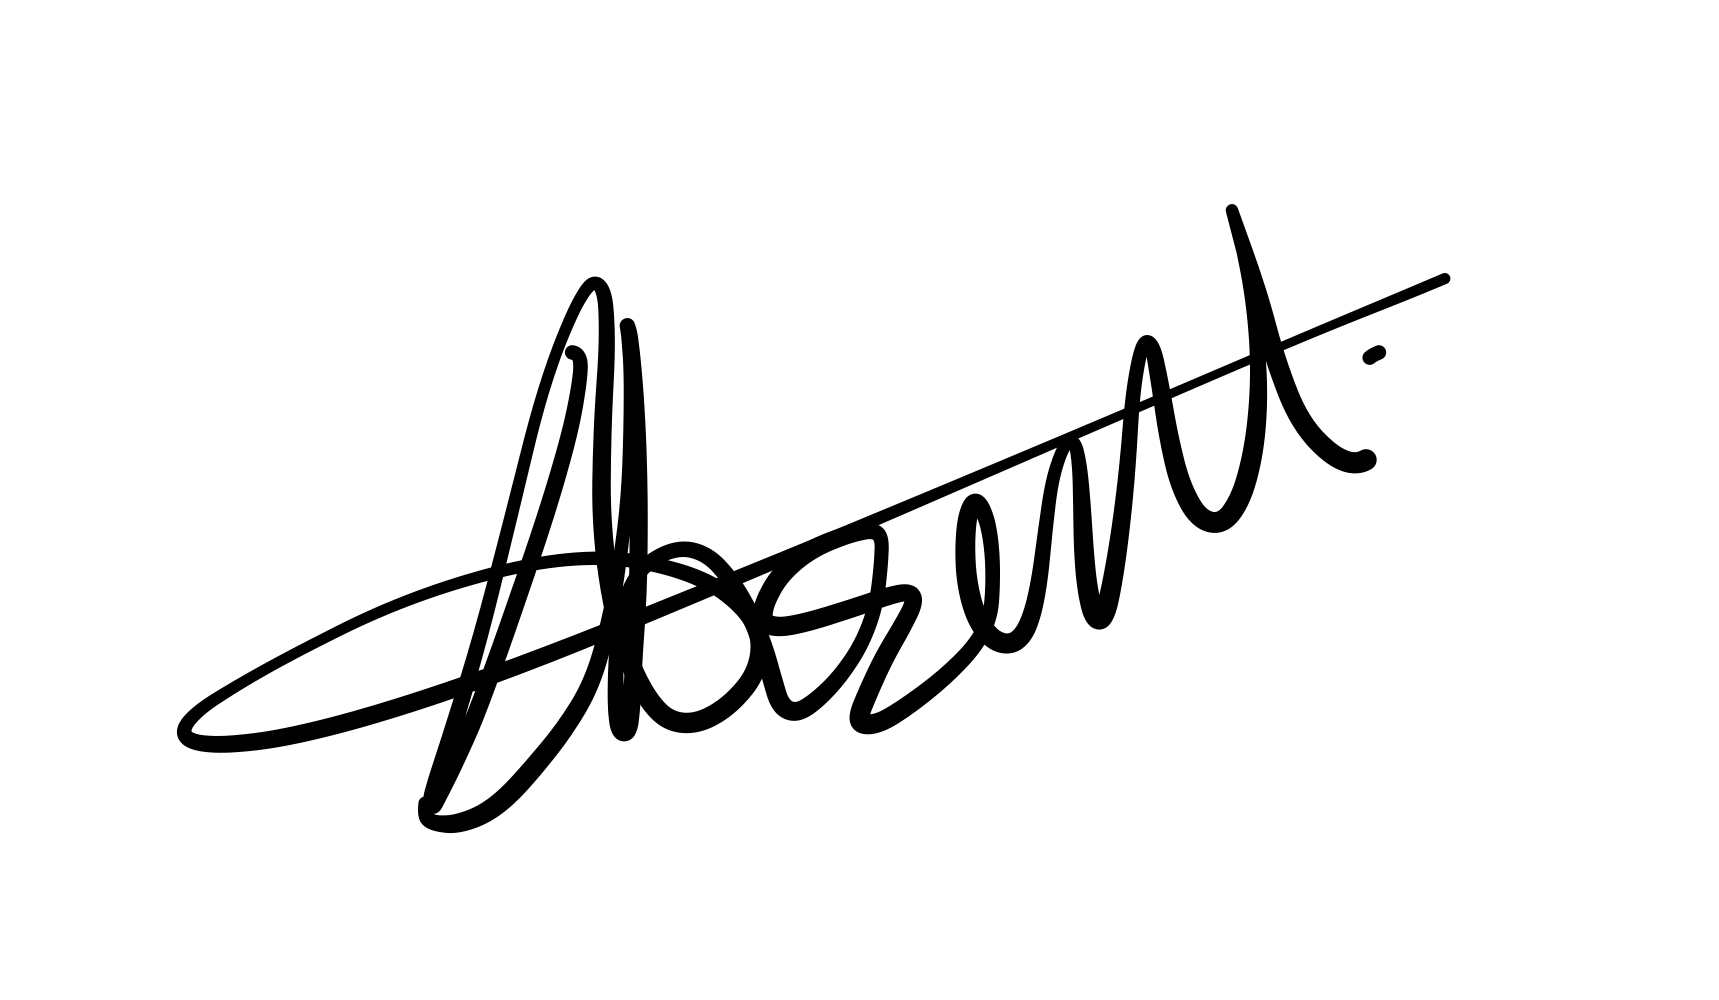
\includegraphics[scale=0.1]{ahsan.jpeg}
        \end{center}
\end{itemize}

\subsection{Rebecca Di Filippo}
\begin{itemize}
  \item Wrote Section 1.1: Purpose of Document
  \item Wrote Section 1.2:  System Description
  \item Wrote Section 1.3: Overview of Document
  \item Contributed 4 Class Responsibility Cards
        \begin{itemize}
          \item Registration
          \item Login
          \item Account Information
          \item View Account
        \end{itemize}
        \begin{center}
          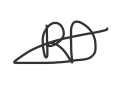
\includegraphics[scale=1.2]{rebecca.png}
        \end{center}
\end{itemize}

\subsection{Ethan Walsh}
\begin{itemize}
  \item Section 3: Derived initial system diagram.
  \item Section 3: Proposed edits to updated system diagram.
  \item Section 3: Wrote initial description of system architecture
  \item Section 3: Wrote description of used architecture styles and rationale
  \item Section 3: Wrote part of section 3.2, Subsystems
  \item Contributed 4 Class Responsibility Cards
        \begin{itemize}
          \item Experts Process Management
          \item Edit Account
          \item Request Information
          \item Account Error
        \end{itemize}
        \begin{center}
          
\includegraphics[scale=0.7]{ethan.png}
        \end{center}
\end{itemize}

\subsection{Jake Finlay}
\begin{itemize}
  \item Came up with some classes for the initial Analysis Class Diagram
  \item Contributed 9 Class Responsibility Cards
        \begin{itemize}
          \item Experts Service
          \item Point System Algorithm Expert
          \item External API Service Expert
          \item Redbook API
          \item AI Expert
          \item AI API
          \item Deal Report Management
          \item View Car Deal Report
          \item Save Car Deal Report
        \end{itemize}
  \item Helped with conversion to Latex
        \begin{center}
          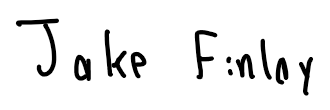
\includegraphics[scale=0.6]{jake.png}
        \end{center}
\end{itemize}

\subsection{Omer Karo}
\begin{itemize}
  \item created initial analysis class diagram for the car recommendation service subsystem
  \item created initial analysis class diagram for the deal report management subsystem
  \item created initial analysis class diagram for the experts process management
  \item Contributed 4 Class Responsibility Cards
        \begin{itemize}
          \item Request Intake
          \item Response Handler
          \item Car Recommendation service
          \item Request Car Depreciation Curve
        \end{itemize}
  \item Helped with conversion to Latex
        \begin{center}
          
\includegraphics[scale=0.2]{omer.jpg}
        \end{center}
\end{itemize}

\subsection{Abdallah Alqashqish}
\begin{itemize}
  \item Section 2: Collaborated on the Analysis Class Diagram (created and determined initial functionality of)
        \begin{itemize}
          \item Account Management Controller.
          \item Experts service.
          \item Refactored experts that depend on API to use a controller and boundary.
        \end{itemize}
  \item Section 3.1: Refined system architecture diagram to match the final agreed upon architecture.
  \item Contributed 4 Class Responsibility Cards
        \begin{itemize}
          \item Car Recommendation Information (Entity).
          \item Account Management (Controller).
          \item Logout (Boundary).
          \item Account Success (Boundary).
        \end{itemize}
        \begin{center}
          
\includegraphics[scale=0.1]{abdallah.jpg}
        \end{center}
\end{itemize}
% End Section


\end{document}
%------------------------------------------------------------------------------